\documentclass[tikz,border=10pt]{standalone}
\begin{document}
\tikzset{
    pics/blocked/.style={
        code={
            \draw[blue] (0,0) foreach \i in {1,...,5} { -- ++ (18-36*\i:0.3) -- ++ (18-36*\i:0.1) -- ++ (0:0.2) };
        }
    },
}
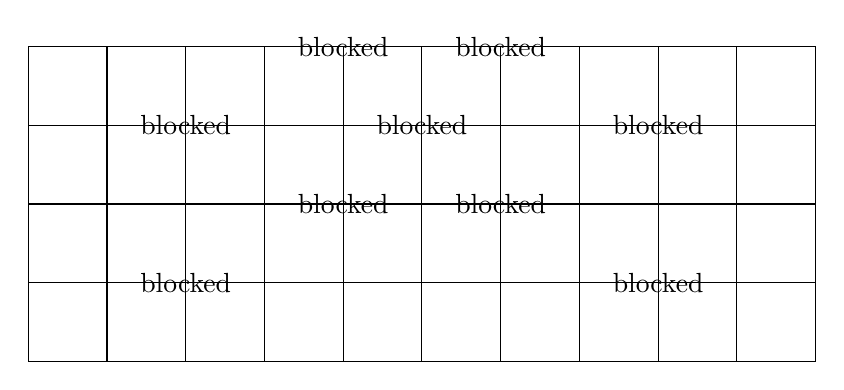
\begin{tikzpicture}
    \fill[red!30] (-5,-3) rectangle (-3,-1);
    \fill[red!30] (-3,-3) rectangle (-1,-1);
    \fill[red!30] (-5,-1) rectangle (-3,1);
    \fill[red!30] (-3,-1) rectangle (-1,1);
    \fill[white] (-5,-3) rectangle (5,1);
    \draw (-5,-3) grid (5,1);
    \node at (0,0) [pic actions] {blocked};
    \node at (1,-1) [pic actions] {blocked};
    \node at (-1,-1) [pic actions] {blocked};
    \node at (1,1) [pic actions] {blocked};
    \node at (-1,1) [pic actions] {blocked};
    \node at (-3,-2) [pic actions] {blocked};
    \node at (-3,0) [pic actions] {blocked};
    \node at (3,-2) [pic actions] {blocked};
    \node at (3,0) [pic actions] {blocked};
\end{tikzpicture}
\end{document}